%
% File emnlp2020.tex
%
%% Based on the style files for ACL 2020, which were
%% Based on the style files for ACL 2018, NAACL 2018/19, which were
%% Based on the style files for ACL-2015, with some improvements
%%  taken from the NAACL-2016 style
%% Based on the style files for ACL-2014, which were, in turn,
%% based on ACL-2013, ACL-2012, ACL-2011, ACL-2010, ACL-IJCNLP-2009,
%% EACL-2009, IJCNLP-2008...
%% Based on the style files for EACL 2006 by 
%%e.agirre@ehu.es or Sergi.Balari@uab.es
%% and that of ACL 08 by Joakim Nivre and Noah Smith

\documentclass[11pt,a4paper]{article}
\usepackage[hyperref]{emnlp2020}
\usepackage{times}
\usepackage{latexsym}
\renewcommand{\UrlFont}{\ttfamily\small}

\newcommand\qtheta{q_\theta}

\makeatletter
\def\blfootnote{\xdef\@thefnmark{}\@footnotetext}
\makeatother

% This is not strictly necessary, and may be commented out,
% but it will improve the layout of the manuscript,
% and will typically save some space.
\usepackage{microtype}

\usepackage{mystyle}
\usepackage{subcaption} 
\usepackage{todonotes}

% trellis
\usepackage{tikz}%

\usepackage{algorithm}
\usepackage[noend]{algpseudocode}

\usepackage{pgfplots}

%% ADD BACK!!!!!!!!!!!!!!!!!
\aclfinalcopy % Uncomment this line for the final submission
%\def\aclpaperid{0} %  Enter the acl Paper ID here

%\setlength\titlebox{5cm}
% You can expand the titlebox if you need extra space
% to show all the authors. Please do not make the titlebox
% smaller than 5cm (the original size); we will check this
% in the camera-ready version and ask you to change it back.

\newcommand\BibTeX{B\textsc{ib}\TeX}
\newcommand\Emit{\mathbf{O}}
\newcommand\Trans{\mathbf{T}}

\title{Class project: Amortized RSA}

\author{Justin T. Chiu\\
  Department of Computer Science \\
  Cornell Tech \\
  \texttt{jtc257@cornell.edu}\\
}

\date{}
\raggedbottom

\begin{document}
\maketitle
\begin{abstract}
The Rational Speech Acts inference procedure has
been demonstrated to be effective as a model of human 
behaviour in small reference games.
However, the inference procedure is expensive
as it requires considering all possible utterances.
\citet{white2020learning} amortize the cost of inference by
training a language model perform to maximize the objective
the RSA procedure optimizes.
The resulting amortized model displays symptomps of
language drift, where in optimizing the RSA objective
produced utterances are unhuman-like.
We build upon their amortization procedure
by proposing a change to the objective
that prevents language drift.
\end{abstract}

\section{Introduction}
% what is rsa
The Rational Speech Acts (RSA) framework is an inference procedure based on Gricean maxims 
for generating and understanding language in a collaborative setting.
% why is it useful
RSA has had empirical success in small domains, in particular simple reference games
with very limited vocabularies.
RSA is potentially useful beyond these domains as a heuristic for utility maximization.
Extensions of RSA to nontrivial vocabularies requires approximations:
incremental RSA \citep{cohngordon2018pragmatically},
reranking, and/or variational inference \citep{white2020learning}.

We focus on amortization for approximating RSA speakers,
which has had empirical success in applications such as 
variational autoencoders and reinforcement learning.
We highlight two broad classes of errors in text generation,
and examine their effects on the \textsc{ShapeWorld} dataset:
model error and search error.

\section{Related Work}
The approach of \citet{white2020learning} is the basis of our project,
and the apply the amortization approach to both the \textsc{ShapeWorld}
and \textsc{Colors} dataset.
Unfortunately we only have time to fit in the \textsc{ShapeWorld} dataset,
on which we find a small contradiction to one of claims:
we find that RSA does not help with task performance.

A similar amortization approach can also be found in \citet{gu2017trainable},
which attempt to train a greedy decoder to mirror the performance
of beam search in a teacher model for machine translation.

Amortization also shows up in variational autoencoders,
and one could interpret all parameterized policies trained through via policy gradient 
as instances of amortization as well,
where the alternative would be to explicitly perform policy iteration.

Incremental RSA \citep{cohngordon2018pragmatically} is another approach 
for approximating the expensive inference procedure in RSA,
although that methods has no principled interpretation.

Approximations for RSA listeners, rather than speakers, have been explored as well.
Other works use a margin-based approximation of pseudolikelihood \citep{gulordava2020dax},
and learn through approximate RSA procedure via importance sampling over utterances
\citep{mcdowell2019learning}.


\section{Problem Setup}
The \textsc{ShapeWorld} dataset consists of games where two players,
a speaker and a listener, collaborate to identify a target object out of a given set.
Given a set of three objects, $o = \set{o_1,o_2,o_3}$, the goal of the speaker
is to accurately describe the object at index $t\in [3]$,
to the listener through a single utterance
$u = \langle u_1, \ldots, u_L \rangle$.
Utterances are limited to a fixed vocabulary of size 14 consisting of colors and shapes.
The data generating process only uses at most $L \le 2$ utterances,
consisting of a color and/or shape.
The literal speaker is a distribution over utterances $s_0 = p(u \mid t, o)$, while
the literal listener is a distribution over targets $l_0 = p(t \mid u, o)$.

\section{Method}
We are interested in decoding an utterance $u$ that refers to target $t$ 
by optimizing the following program:
\begin{equation}
\argmax_u F(u, t, o),
\end{equation}
where $F$ is only able to score full utterances $u$.
This prevents efficient inference, which would require that $F$
decomposes over prefixes of $u$ from left to right.
Such a decomposition would allow beam search, or other approximate inference techniques.
Instead, we must optimize $F$ with the following procedure:
\begin{enumerate}
\item Enumerate all possible utterances $u$
\item Score all utterances according to $F(u,t,o)$
\item Choose the highest scoring utterance.
\end{enumerate}
When the number of possible utterances is infinite or exponentially large
in the length of the longest allowed utterance, this procedure is infeasible.

Rather than decoding by enumerating all possible sequence for each context,
\citet{white2020learning} propose to amortize the cost of inference.
This is accomplished by training a left-to-right model to approximate the argmax of $F$
by optimizing the following program:  
\begin{equation}
\argmax_\theta \Es{p(t,o)}{\Es{q_\theta(u\mid t,o)}{F(u,t,o)}},
\end{equation}
where $q_\theta(u \mid t, o)$ is the amortized speaker.
This objective can be optimized via stochastic gradient descent using the 
score function gradient estimator, or a biased gradient estimator in the Gumbel-softmax
family of estimators.

\citet{white2020learning} explore a single objective, given by
\begin{equation}
F_{\textrm{length}}(t,u,o) = \log l_0(t\mid u,o)  + \log \lambda|u|.
\end{equation}
This corresponds to MAP inference in a noisy channel model with
a relatively uninformative prior that is constant given a length.
The hyperparameter $\lambda$ controls how much influence the prior has on the objective.
We refer to this objective as length.

We explore two more objectives, the first of which uses an informative prior in MAP inference:
\begin{equation}
F_{\textrm{MAP}}(t,u,o) = \log l_0(t\mid u,o) + \log p(u\mid o),
\end{equation}
where $p(u \mid o)$ is a speaker that does not condition on the target $t$.
We refer to this objective as MAP.

The last objective introduces a slightly larger change.
Rather than approximate MAP inference,
the goal is to fully approximate the posterior of the following noisy channel model
$$p(u \mid t,o) = \frac{p(t \mid u, o)p(u \mid o)}{p(t \mid o)}.$$
This is accomplished by minimizing the KL divergence between the posterior
and the amortized approximation as follows:
\begin{equation}
\label{eqn:bayes}
\begin{aligned}
&\min_\theta \KL{\qtheta(u\mid t) \;||\; p(u\mid t)}\\
&= \min_\theta \Es{\qtheta(u)}{\log \qtheta(u\mid t) - \log p(u\mid t)}\\
&= \min_\theta \Es{\qtheta(u)}{\log \qtheta(u\mid t) - \log p(t \mid u)p(u)},
\end{aligned}
\end{equation}
where conditioning on the full context $o$ has been dropped for brevity,
and the denominator $p(t\mid o)$ from the posterior is constant wrt $\theta$
and can be safely ignored.
We refer to this objective as Bayes.

The difference between the MAP and Bayes objectives is the addition of 
the negative entropy term, $\Es{q}{\log q}$, in Equation~\ref{eqn:bayes}.
This entropy regularization encourages $q$ to not reduce to a point mass,
unlike the other objectives which have no such pressure.

\section{Experiments}
We evaluate amortized speakers obtained by optimizing the 
three objectives: length, MAP, and Bayes, on the \textsc{ShapeWorld} dataset.
We compare the three amortized speakers against each other, as well as against
the base literal speaker, on three metrics:
how accurately a collection of literal listeners trained on separate data
can infer the correct target,
the likelihood of the produced utterances under a marginal language model,
and the length of the produced utterances.
The last two metrics, likelihood and length, are strongly correlated in the case of 
\textsc{ShapeWorld}, where there is no strong preference for particular utterances
due to the small size of the vocabulary.

Literal listeners and speakers are trained on the same splits of randomly sampled
\textsc{ShapeWorld} contexts as in \citep{white2020learning}.
The speaker $p(u \mid o)$ that was used to train the amortized speakers and
does not conditional on targets was trained on the same training splits.
Amortized speakers are trained via stochastic gradient descent using the
straight-through Gumbel-softmax gradient estimator.

Ten test literal listeners were trained on held-out generated data and used for evaluation.

\section{Results}
Before discussing speaker performance,
we find that the base literal listener is quite accurate, obtaining 96.94\% accuracy
on the ground truth test data.
This is expected, as the data in \textsc{ShapeWorld} is very simple and artificially generated.


\begin{figure}[t]
\centering
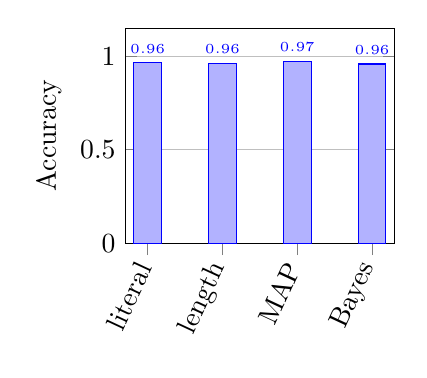
\begin{tikzpicture}
\begin{axis}[
    ybar=5pt,
    ylabel=Accuracy,
    symbolic x coords={literal, length, MAP, Bayes},    
    nodes near coords,
    nodes near coords align={vertical},
    every node near coord/.append style={font=\tiny},
    width=5cm,
    xtick pos=left,
    ymajorgrids=true,
    ymin=0,
    ymax=1.15,
    xticklabel style={rotate=65, anchor=east},
]
\addplot coordinates {
    (literal, 0.9648)
    (length, 0.9636)
    (MAP, 0.9724)
    (Bayes, 0.9588)
};
\end{axis}
\end{tikzpicture}
\caption{The speaker accuracies using an ensemble of listeners trained on
held out data for \textsc{ShapeWorld}.
The literal speaker was trained directly via MLE, while the amortized
length, MAP, and Bayes speakers were trained to optimize their
eponymous objectives using the straight-through Gumbel-softmax estimator.
}
\label{fig:accuracy}
\end{figure}

\begin{figure}[t]
\centering
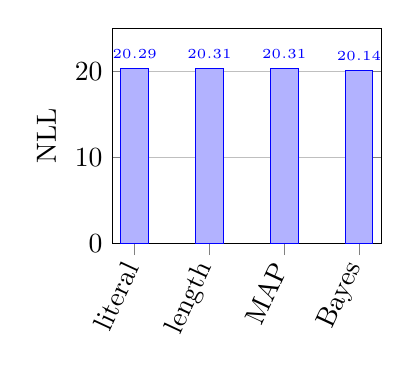
\begin{tikzpicture}
\begin{axis}[
    ybar=5pt,
    ylabel=NLL,
    symbolic x coords={literal, length, MAP, Bayes},    
    nodes near coords,
    nodes near coords align={vertical},
    every node near coord/.append style={font=\tiny},
    width=5cm,
    xtick pos=left,
    ymajorgrids=true,
    ymin=0,
    ymax=25,
    xticklabel style={rotate=65, anchor=east},
]
\addplot coordinates {
    (literal, 20.288)
    (length, 20.31)
    (MAP, 20.3076)
    (Bayes, 20.1356)
};
\end{axis}
\end{tikzpicture}
\caption{The average negative log likelihood (NLL) of utterances produced from each speaker in
\textsc{ShapeWorld} as measured by a marginal language model $p(u)$ that
does not see the objects or target.
The lower the NLL, the better.
}
\label{fig:likelihood}
\end{figure}


\begin{figure}[t]
\centering
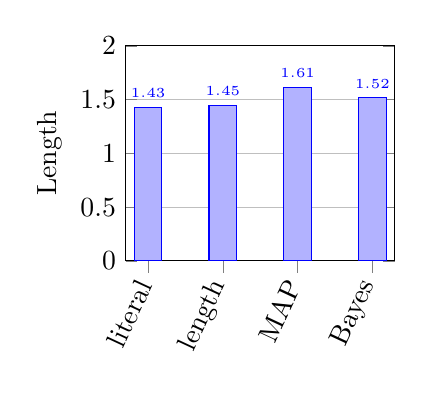
\begin{tikzpicture}
\begin{axis}[
    ybar=5pt,
    ylabel=Length,
    symbolic x coords={literal, length, MAP, Bayes},    
    nodes near coords,
    nodes near coords align={vertical},
    every node near coord/.append style={font=\tiny},
    width=5cm,
    xtick pos=left,
    ymajorgrids=true,
    ymin=0,
    ymax=2,
    xticklabel style={rotate=65, anchor=east},
]
\addplot coordinates {
    (literal, 1.4256)
    (length, 1.448)
    (MAP, 1.6132)
    (Bayes, 1.5158)
};
\end{axis}
\end{tikzpicture}
\caption{The average utterance lengths from each speaker using
an ensemble of listeners trained on
held out data for \textsc{ShapeWorld}.
}
\label{fig:length}
\end{figure}

As for speaker performance, we find that all speakers are very accurate
and obtain at least 96\% accuracy when evaluated with test literal listeners
trained on held-out data, as shown in Figure~\ref{fig:accuracy}.
The MAP speaker outperformed the other variants very slightly.
We additionally outperform the speakers from \citet{white2020learning},
where the literal speaker obtained 73\% accuracy.

The likehoods of the utterances produced by the speaker also is very close,
as shown in Figure~\ref{fig:likelihood}.
Interestingly, the Bayes speaker has slightly better likelihood.
This is surprising, as there is little difference between the MAP and Bayes
objectives. It is likely that this is not statistically significant.

The average lengths of the utterances of the speakers is given in Figure~\ref{fig:length}.
The MAP utterances are on average longest.
This may account for the higher accurace of the MAP speaker, which could be producing
longer utterances resulting in less ambiguity.
Since the MAP objective has an informative utterance prior, this leads to less
pressure to produce shorter utterances.

The observation that the MAP speaker has higher accuracy as well as longer utterances
implies that the literal speaker underestimates the listener, and occasionally
does not provide enough information in an utterance.
This could happen in a scenario where both the color and shape is necessary to 
successfully communicate a shape, but only one of the two qualities is uttered.

\section{Discussion}
Unfortunately, the \textsc{ShapeWorld} dataset itself is too simple to observe
language drift, leaving our study inconclusive as to whether the proposed
method fixes that particular issue.
However, we may return shortly with results on the \textsc{Colors} dataset,
which did exhibit speakers with language drift.

Additionally, it noteworthy that application of the straight through Gumbel-softmax
estimator may be leading to extremely unstable learning dynamics.
Although the objective improves for the first few epochs,
performance on the training objective eventually plummets.

\bibliographystyle{acl_natbib}
\bibliography{anthology}

%\clearpage
%\appendix

%\section*{Appendix}
%\section{Blah}
   
\end{document}
